\documentclass [9 pt]{article}
\usepackage[margin = 1in]{geometry}
\usepackage{amsfonts}
\usepackage{amsthm}
\usepackage{bbm}
\usepackage{amsmath}
\usepackage{arydshln}
\usepackage[utf8]{inputenc}
\usepackage{graphicx}
\usepackage{enumerate}
\usepackage{color}
\usepackage[dvipsnames]{xcolor}
\usepackage{graphicx}
\graphicspath{ {./images/} }
\usepackage{tikz}
\usepackage{xcolor}
\usepackage{listings}
\usepackage{color}

\definecolor{dkgreen}{rgb}{0,0.6,0}
\definecolor{gray}{rgb}{0.5,0.5,0.5}
\definecolor{mauve}{rgb}{0.58,0,0.82}


\lstset{
  language=Matlab,
  basicstyle=\ttfamily,               
  numbers=left,                  
  stepnumber=1,                  
  numbersep=5pt,                  
  backgroundcolor=\color{white}, 
  showspaces=false,              
  showstringspaces=false,        
  showtabs=false,                
  tabsize=2,                     
  captionpos=b,                  
  breaklines=true,               
  breakatwhitespace=true,         
  title=\lstname,
  numberstyle=\tiny\color{Black},
  keywordstyle=\color{BrickRed},
  commentstyle=\color{dkgreen},
  stringstyle=\color{mauve},  
}

\theoremstyle{definition}
\newtheorem{problem}{Problem}
\newtheorem{theorem}{Theorem}
\newtheorem*{corollary}{Corollary}
\newtheorem{proposition}[theorem]{Proposition}
\newtheorem{lemma}[theorem]{Lemma}
\newtheorem{conjecture}[theorem]{Conjecture}

\newtheorem{definition}[theorem]{Definition}
\newtheorem{remark}[theorem]{Remark}
\newtheorem{example}[theorem]{Example}


\usepackage{fancyhdr}
\pagestyle{fancy}
\lhead{Yuhao Wu \quad 260711365} 
\rhead{\bfseries COMP 350 Midterm Review 1}
\cfoot{\thepage}
\renewcommand{\headrulewidth}{0.4pt}
\renewcommand{\footrulewidth}{0.4pt}


\setlength{\parindent}{0pt}


\begin{document}
\section*{IEEE Floating Points}
\textbf{Single Format: (32)}
$$ \pm \ | \ a_1, a_2, \ldots a_8 \ |\ b_1, b_2, \ldots b_{23}$$
$\pm$ refers to the sign, 0 for positive, 1 for negative
\\
\\
\textbf{Double Format: (64)}
$$ \pm \ | \ a_1, a_2, \ldots a_{11} \ |\ b_1, b_2, \ldots b_{52}$$
\\
\\
Hidden bit normalization: don't store $b_0$, as we know $b_0 = 1$\\
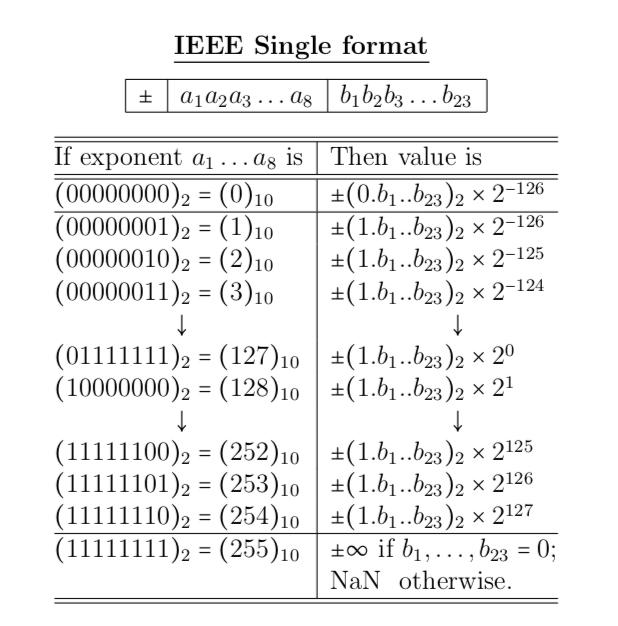
\includegraphics{1}
\\
\\
The exponent representation $a_1, a_2, \ldots, a_8$ uses \textbf{biased representation}: this bit-string is the binary presentation of $E + 127$. 127 is the \textbf{exponent bias}. 
$$127 = (111111110)_2 / 2 = (2^8 - 1 - 1) / 2 = 127$$
\begin{itemize}
	\item \textbf{Smallest positive normal number} is 
	$$  (1.00\ldots 0)_2 \times 2^{-126}  $$
	$$  0 \ | \ 0 0 \ldots 1 \ |\ 00000 \ldots 0  $$
	\item \textbf{Largest positive normal number} is 
	$$  (1.11\ldots 1)_2 \times 2^{127}  $$
	$$  0 \ | \ 1 1 \ldots 1 0 \ |\ 1111 \ldots 1  $$
\end{itemize}





\newpage
\subsection*{Subnormal Numbers:}
\textbf{Subnormal Numbers} are in the form:
$$ 0.b_1b_2, \ldots b_{23} \times 2^{-126} $$\\
\textbf{Smallest Positive number we can store:}
$$ 0 \ |\ 000 \ldots 0 \ |\  000000 \ldots 01  = 2^{-23} \times 2^{-126} =  2^{-149}$$\\
Subnormal numbers can't be normalized as the exponent field won't fit.\\
Subnormal numbers have less accuracy as the less room for non-zero bits in the fraction.



\subsection*{$\pm \infty$ and NaN:}
This shows an exponent bit-string of all ones is a special pattern for $\pm \infty$ or NaN, depending on the value of the fraction.\\
if $ b_1  = b_2 = \ldots = b_{23} = 0 \implies \pm \infty $\\
\newline
a quite $NaN$ (qNaN) if $b_1 = 1$ and a signalling $NaN$
 (sNaN) if $ b_1 = 0 $.


\subsection*{Machine Epsilon:}
\textbf{Definition}: The \textbf{gap} between the number \textbf{1} and \textbf{the next larger} floating point number is called the machine epsilon of the floating point system, denoted by $\varepsilon$.\\
\newline
The number of bits in the significant (including the hidden bit) is called the \textbf{ precision of the floating point system }, denoted by $p$.
\newline
\newline
In the \textbf{single format} system, the number after 1 is
$$   b_0\ . \ b_1 b_2 b_3 \ldots b_{23} = 1\ .\ 000 \ldots 1 $$
So, Machine Epsilon is $2^{-23}$\\
\newline\newline
In the \textbf{double format} system, the number after 1 is
$$   b_0\ . \ b_1 b_2 b_3 \ldots b_{52} = 1\ .\ 000 \ldots 1 $$
So, Machine Epsilon is $2^{-52}$\\
\newline
\textbf{GAP:}\\
Let $x=m\times 2^E$ be a single format number with $1 \leq m < 2$. The gap between $x$ and the next single format number is
$$ \varepsilon \times 2^E $$

\newpage
\subsection*{Rounding:}
\begin{itemize}
	\item Round down: $round(x) = x_{-}$
	\item Round up: $round(x) = x_{+}$
	\item Round towards zero: $round(x)$ is either $x_{-}$ or $x_{+}$, whichever is between zero and x.
	\item Round to nearest: $round(x)$ is either $x_{-}$ or $x_{+}$, whichever is nearer to $x$.\\
	 In the case of a tie, the one with \textbf{ its least significant bit equal to zero } is chosen

\end{itemize}

\subsection*{Absolute Rounding Error:}
\textbf{Definition:} The absolute rounding error associated with $x$:
$$ | round(x) - x | $$
For all modes, we obviously have $ | round(x) - x | < |x_{+} - x_{-}|  $\\
\\
Suppose $N_{min} \leq x \leq N_{max}$,
$$x=(b_0.b_1b_2\ldots b_{22}b_{23}b_{24}b_{25} \ldots )_2 \times 2^E, b_0=1$$.
$$ \text{ IEEE single } x_{-} = (b_0.b_1b_2\ldots b_{22}b_{23} )_2 \times 2^E, b_0=1   $$
$$ \text{ IEEE single } x_{+} = x_{-} + 0.00 \ldots 001 \times 2^E $$
So for any mode:
$$ | round(x) - x | < |x_{+} - x_{-}| = 0.00 \ldots 001 \times 2^E = 2^{-23} \times 2^E  = \epsilon \times 2^E $$
\textbf{ Question: } Is this the same for subnormal numbers?



\subsection*{Relative Rounding Error: }
\textbf{Definition:} The \textbf{relative rounding error} is defined by $|\delta|$, where
$$ |\delta| = |\dfrac{round(x) - x}{x}| $$

\begin{equation}
|\dfrac{round(x) - x}{x}|   \left\{
             \begin{array}{lr}
            < \varepsilon \quad \text{Any mode}\\
			\leq \dfrac{\varepsilon}{2} \quad \text{the nearest}\\ 
             \end{array}
\right.
\end{equation}
\\
\\
\textbf{Question: } How to prove this?\\
\textbf{NOTE:} condition: $x$ is in the normal range

\subsection*{IEEE for Rounded Arithmetic}
$$ x \ominus y = round(x - y) $$
According to the relative rounding errors, we have:
$$ x \ominus y = round(x - y) = (x - y)\cdot (1 + \delta) $$

\subsection*{Exception Cases:}
\begin{itemize}
	\item $\dfrac{a}{0} \implies \infty$
	\item $a \times \infty \implies \infty$
	\item  $a + \infty \implies \infty$ 
	\item $a - \infty \implies  -\infty$ 
	\item $\dfrac{a}{ \infty} \implies 0$
	\item  $\infty + \infty \implies \infty$ 
	\item $ \infty \times 0 \implies NaN $
	\item $\dfrac{0}{0} \implies NaN$
	\item $\dfrac{\infty }{ \infty} \implies NaN$
	\item $\infty - \infty \implies NaN$ 
\end{itemize}
We stated before that there are two types of NaN: qNaN and sNaN. Their only difference is that sNaN generates interruption while qNaN does not. The application decides if it generates qNaN or sNaN. 

\subsection*{Overflow and Underflow:}
\textbf{Overflow} is said to occur when
$$ N_{max} < |\text{ true result }| < \infty $$
where $N_{max}$ is the largest normal FPN.\\
\newline
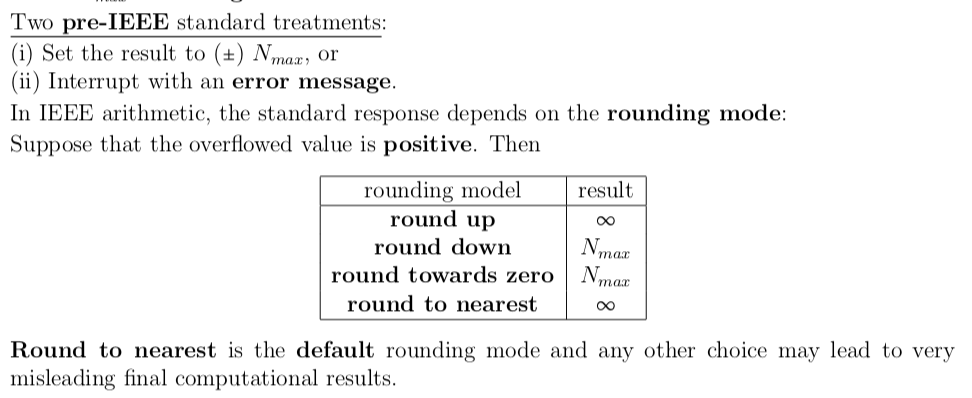
\includegraphics{2}

\newpage
\textbf{Underflow} is said to occur when
$$ 0 < |\text{ true result }| < N_{min} $$
where $N_{min}$ is the minimum normal FPN.\\
\newline
\newline
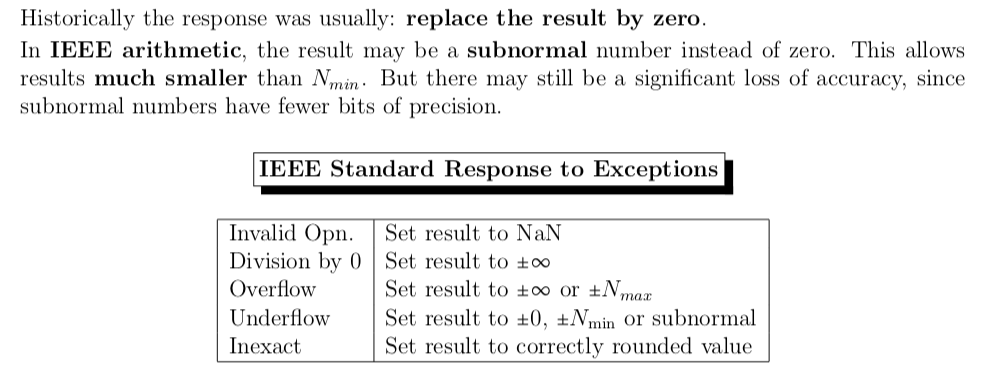
\includegraphics{3}




\end{document}